%%% LaTeX Template: Article/Thesis/etc. with colored headings and special fonts
%%%
%%% Source: http://www.howtotex.com/

\documentclass[12pt]{article}


\usepackage{apuntes-estilo}
\usepackage{fancyhdr,lastpage}
\usepackage{color,colortbl}
\usepackage{verbatim}

\def\maketitle{

% Titulo 
 \makeatletter
 {\color{bl} \centering \huge \sc \textbf{
 Procesos \\ 
\large \vspace*{-8pt} \color{black} Guía básica de administración de procesos. 
 \vspace*{8pt} }\par}
 \makeatother


% Autor
 \makeatletter
 {\centering \small 
 	Departamento de Ingeniería de Computadoras \\
 	Facultad de Informática - Universidad Nacional del Comahue \\
 	\vspace{20pt} }
 \makeatother

}

% Custom headers and footers
\fancyhf{} % clear all header and footer fields
\fancypagestyle{plain}{\fancyhf{}}
  	\pagestyle{fancy}
 	\lhead{\footnotesize Administración de procesos - Departamento de Ingeniería de Computadoras}
 	\rhead{\footnotesize \thepage\ }	% ''Page 1 of 2''

\def\ti#1#2{\texttt{#1} & #2 \\ }



\begin{document}

\thispagestyle{empty}
\maketitle
\setlength{\parindent}{0pt}

\section*{Introducción}

Hemos hablado durante un apunte anterior acerca de reconocimiento de 
recursos físicos, identificar sus características y representación dentro 
del sistema operativo. Durante el próximo texto hablaremos de 
monitorear el consumo de recursos por parte de los proesos en ejecución. 
Por este motivo, durante el presente apunte se desarrollarán conceptos y 
procedimientos relacionados a la administración de procesos, como una 
instancia previa a evaluar el consumo de recursos por parte de los mismos.

Es decir, no podemos evaluar el consumo de recursos por parte de los
procesos, sin conocer mínimamente las actividades báscias de administración
que se realizan sobre los mismos. 


\section*{Procesos}

Un proceso es un programa en ejecución. Son digamos, las entidades vivas 
dentro de nuestro sistema. Cada programa que ejecutamos, por ejemplo el 
navegador web, puede disparar la ejecución de uno o mas procesos para 
llevar a cabo su tarea.  A su vez, existen procesos que no son disparados 
por los usuarios, sino que los ejecuta el sistema operativo en sí mismo 
para cumplir sus funciones. Por ejemplo, el proceso \texttt{init}, ó el 
servicio de ssh. 

Los procesos en ejecución necesitan consumir recursos computacionales para 
llevar a cabo su función: CPU, memoria principal (RAM), memoria secundaria, 
transferir datos por red, etc. Algunos procesos necesitarán más tiempo de 
CPU, como puede ser un juego, o un programa de calculo; mientras que 
otros, por ejemplo el web browser, necesitarán más memoria principal 
(RAM), etc.

Es la intención de este apunte observar el consumo de recursos por parte de 
los procesos en ejecución. 
 
\subsection*{Estado de los procesos}

El orden en que los procesos reciben la atención de el CPUs, es 
similar a lo que ocurre con las cajas de cobro en un supermercado. 
Imaginemos que cada caja de cobro es un CPU y las personas son los 
procesos. Al igual que en el supermercado, las colas se organizan con 
prioridades, de modo que algunos procesos pueden tener prioridad 
sobre otros a la hora de ser atendidos por el CPU. 

Los procesos no siempre se encuentran en ejecución. 
Como bien sabemos, la cantidad de CPUs disponibles es finita, por ende 
los procesos compiten por 
pequeñas porciones de tiempo de CPU. Momento en el cual, el proceso en 
ejecución tendrá la oportunidad de ejecutar algunas instrucciones de su 
código, hasta en tanto se acabe su porción de tiempo de CPU o bien ocurra 
algún otro evento que evite que el proceso se siga ejecutando (por ejemplo, 
porque está esperando recibir datos de la red). 

Si un proceso necesita abrir un archivo que se encuentra en 
memoria secundaria (disco), habrá una pequeña cantidad de tiempo en la que 
dicho proceso estará esperando por la respuesta del disco, que es muchas 
veces más lenta que la velocidad de procesamiento del CPU. Durante esta
espera, el proceso no está listo para ser ejecutado en CPU, se encuentra 
``durmiendo''. Por lo que, mientras el proceso espera, otros procesos 
pueden aprovechar y ejecutarse en el CPU. 
  
Es así que durante el tiempo de vida de un proceso, este se encontrará en 
diferentes estados. En un sistema GNU/Linux observaremos básicamente 
cinco posibles estados, observables por el administrador de sistemas: 

\begin{itemize}
\item R = Corriendo (running): significa que el proceso se encuentra en 
condiciones de ejecutarse en CPU o bien que está siendo ejecutado.  
\item S = Durmiendo (sleeping): el proceso se encuentra esperando por 
alguna señal o evento, no se encuentra en condiciones de ser ejecutado en 
CPU al momento. 
\item T = Trazado o detenido (traced or stopped): proceso que ha recibido 
la orden de detenerse (por ejemplo a pedido del usuario con el comando 
kill y la señal SIGSTOP). 
\item D = Durmiendo no interrumpible (uninterruptible sleep): se encuentra
esperando por un evento y no puede ser interrumpido. 
\item Z = zombie: proceso que termino y no fue reclamado por su proceso 
padre. 
\end{itemize}

Las transiciones entre estados siguen el siguiente esquema: 

\begin{center}
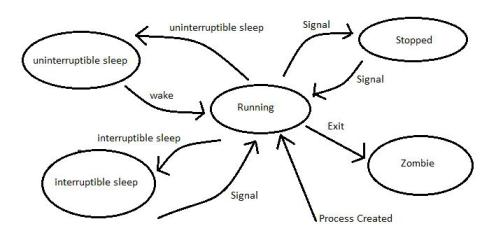
\includegraphics{process-states-s.jpg}
\end{center}
 
Estas transiciones serán en la mayoría de los casos generadas por la misma
funcionalidad del programa, es decir cuando necesita abrir un archivo
estará en estado S, cunado necesita ejecutarse estará en estado R, etc. 
Es decir, el administrador de sistemas, en general no interviene en las
transiciones de estados. Sin embargo, hay casos en los que esto ocurre. 

\subsection*{Manipulación de procesos}

En el uso cotidiano de un sistema de escritorio, el usuario interviene 
en los estados de los procesos sin darse cuenta. Al pedirle a un programa
que se cierre (por ejemplo apretando la ``X'' en la ventana), el usuario
le esta pidiendo al proceso que termine y deje de existir. 

El administrador de sistemas en ocasiones deberá manipular el estado de 
los procesos con diferentes fines. Para ello, enviará señales a los 
mismos a través del comando \texttt{kill}. 

\fcolorbox{black}{grey}{
\parbox[t]{1.0\linewidth}{ \vspace*{0.4cm}
{\bf Importante}: cada proceso tiene un usuario dueño (el nombre del
 usuario dueño se observa en la primer columna de la salida de 
\texttt{ps -ef}). El envío de señales a un proceso mediante el 
comando \texttt{kill} sólo podrá realizarlo el dueño o \textbf{root}
\vspace*{0.4cm} } }

El comando \texttt{kill} (matar) tiene una funcionalidad predeterminada, 
equivalente a cerrar un programa desde la interfase gráfica, esto es envía
al proceso la señal SIGTERM (15). El comando 
recibe como argumento una señal y un identificador de proceso (PID) al 
cual enviarle la señal. 

\colorbox{grey}{\parbox[t]{0.95\linewidth}{ \vspace*{0.5cm} { 
{\bf Ejemplo de uso de kill :} \\
{\tt
Sección de la salida del comando \texttt{ps -ef}\\
lechnerm  7324  7320  0 12:40 ?        00:00:00 gnome-pty-helper \\
lechnerm  7325  7320  0 12:40 pts/0    00:00:00 bash\\
lechnerm 10400  7320  0 13:11 pts/2    00:00:00 bash\\
www-data 10725  4250  0 13:12 ?        00:00:00 /usr/sbin/apache2 -k start \\
}
Si, observando la salida anterior, ejecutamos ``\texttt{kill 10725}'', 
estaremos pidiéndole al programa apache2 que termine su ejecución. 
} \vspace*{0.5cm} } } 
	
El comando \texttt{kill} permite, además de su funcionalidad predeterminada,
enviar otras señales que generan otros cambios de estado diferentes al de 
terminar. La lista de señales posibles se pueden listar observando la 
salida del comando \texttt{kill -l}. La explicación particular de cada 
una de ellas se puede encontrar en la sección siete de las paginas del 
manual online página ``signal'' (\texttt{man 7 signal}).  

Cada señal tiene un número y un nombre en mayúsculas asociado, cualquiera
de ellos puede utilizarse como argumento del comando \texttt{kill}  
En particular hablaremos de las señales mas frecuentemente utilizadas: 
SIGSTOP (19), SIGCONT(18), SIGTERM (15) y  SIGKILL (9).  

\textbf{SIGTERM (15) - Predeterminada}

La señal SIGTERM es la predeterminada al utilizar el comando kill. Esto 
es, si ejecutamos el comando kill utilizando sólo como argumento el PID 
de un proceso, le estaremos enviando SIGTERM. Esto significa que le estamos
pidiendo \textit{amablemente} al proceso que finalice su ejecución. 
Si el proceso puede responder a esta señal, ejecutará instrucciones de 
cierre (como por ejemplo cerrar archivos abiertos) y finalizará su 
ejecución correctamente liberando los recursos que estaba consumiendo. 

\colorbox{grey}{\parbox[t]{0.95\linewidth}{ \vspace*{0.5cm} { 
{\bf }
Ejecutar ``\texttt{kill 1232}'' es equivalente a ``\texttt{kill -SIGTERM 
1232}'', y a ``\texttt{kill -15 1232}'' (asumiendo que 1232 es un PID 
válido). 
} \vspace*{0.5cm} } } 

\textbf{SIGKILL (9) - Terminación abrupta}

Muchos administradores de sistemas utilizan esta señal como un estándar, 
esto además de incorrecto es riesgoso. La señal SIGKILL es equivalente en 
intención a SIGTERM, es decir que si enviamos esta señal a un proceso, 
nuestra intención es finalizar al mismo. Sin embargo, en este caso el
cierre no es amable, al enviar la señal SIGKILL el proceso pierde la 
posibilidad de finalizar correctamente y muchos de los recursos que 
utilizaba pueden quedar retenidos por un cierto período de tiempo.  


\fcolorbox{black}{grey}{
\parbox[t]{1.0\linewidth}{ \vspace*{0.4cm}
{\bf Lo importante:} La señal SIGKILL no puede ser desatendida por el 
proceso, mientras que SIGTERM si (el proceso puede no hacer caso al 
pedido de terminación). Es importante primero intentar finalizarlo 
amablemente (SIGTERM) y luego si no responde aplicar SIGKILL. 
\vspace*{0.4cm} } }


\textbf{SIGSTOP (19) - Deteniendo un proceso}

A veces, el administrador no quiere terminar un proceso, pero necesita
que éste detenga su ejecución temporalmente. La señal SIGSTOP, no puede
ser ignorada por los procesos, y realiza exactamente esta función de 
detener la ejecución del mismo. 

Una vez que enviamos esta señal a un proceso, el proceso se encontrará en 
estado detenido ``T''.


\colorbox{grey}{\parbox[t]{0.95\linewidth}{ \vspace*{0.5cm} { 
{\bf Ejemplo:} deteniendo al navegador web iceweasel. \\
{\tt
\# ps -elf|grep iceweasel |grep -v grep \\
0 S lechnerm 19308  3623 10  80   0 - 213762 -     23:49 ?    00:00:06 iceweasel \\

\# kill -SIGSTOP 19308 \\

\# ps -elf|grep iceweasel |grep -v grep \\
0 T lechnerm 19308  3623 14  80   0 - 234269 -     23:49 ?    00:00:08 iceweasel \\
}
Obsérvese el cambio de estado (segundo valor mostrado en la salida de ps), 
de ``S'' a ``T''. 
} \vspace*{0.5cm} } } 


\textbf{SIGCONT (18) - Reactivando un proceso}

La señal SIGCONT permite al administrador indicarle al proceso que debe 
continuar su ejecución. Esta señal tiene sentido luego de haber enviado 
SIGSTOP al proceso. Siguiendo el ejemplo anterior, enviaremos la señal de
continuación, SIGCONT, al navegador web previamente detenido.  


\colorbox{grey}{\parbox[t]{0.95\linewidth}{ \vspace*{0.5cm} { 
{\bf Ejemplo:} reactivando el navegador web. \\
{\tt
\# ps -elf|grep iceweasel |grep -v grep  \\
0 T lechnerm 19308  3623 14  80   0 - 234269 -     23:49 ?    00:00:08 iceweasel \\

kill -SIGCONT 19308 \\

ps -elf|grep iceweasel |grep -v grep  \\
0 S lechnerm 19308  3623 10  80   0 - 213762 -     23:49 ?    00:00:09 iceweasel \\
}
Obsérvese el cambio de estado (segundo valor mostrado en la salida de ps), 
de ``T'' a ``S''. 

} \vspace*{0.5cm} } }

\subsection*{Ejecución en primer y segundo plano}

En Linux proceso puede estar en primer (foreground) o segundo plano
(background). Solo un proceso estará en primer plano al mismo tiempo en
una terminal, y es con el que estemos trabajando e interactuando en ese 
momento. Un proceso que este en segundo plano no recibirá interacción  
de parte nuestra, es decir que no nos podemos comunicar con él 
a través, por ejemplo, del teclado. 

La utilidad de enviar un programa a 
segundo plano esta dada por el hecho de que existen tareas que no 
requieren de nuestro control para que se ejecuten. Por ejemplo, bajar 
algún archivo de Internet, compilar el kernel u otro programa. Estas son 
tareas que pueden ser lanzadas tranquilamente en segundo plano. 

También, cuando el número de terminales disponibles es reducido,  
podemos querer suspender una tarea en la terminal, enviarla a 
segundo plano y ejecutar otras tareas para luego volver a recuperar la 
tarea que mandamos a segundo plano. 

Un programa en foreground lanzado desde una terminal monopoliza dicha
terminal, por lo que en principio, no podremos ejecutar ningún otro 
programa a la vez. 

Por el contrario un programa en background una vez iniciado, deja de 
monopolizar la terminal desde el que se lanzo, y esta nos vuelve a 
mostrar el prompt.

{\bf ¿Cómo ejecutamos un programa en segundo plano desde la terminal? }

Para lanzar un proceso en segundo plano, tendremos que poner a continuación 
del comando el símbolo ``\&''. 


{\bf ¿Cómo podemos ejecutar otro programa desde un terminal con otro
 programa en ejecución en foreground?}

Una vez ejecutado el programa que captura la terminal, pulsamos CTRL+z 
en la misma, con lo que detenemos el programa en ejecución (equivalente
a enviar la señal SIGSTOP). Tenga cuidado, al pausar el programa, este 
dejará de funcionar (estado T, detenido). En este punto recuperamos 
el prompt en la terminal y podemos ejecutar otro comando. 

 Podemos hacer una prueba lanzamos gimp y comprobamos que podemos operar con él, luego pulsamos CTRL-z y vemos como dejamos de poder trabajar con gimp, aunque permanezca abierto. En este momento el prompt en la terminal esta 
esperando por nuevos comandos.  

Ahora queremos volver a poner en funcionamiento a gimp y así poder volver a utilizar gimp, hay dos modos de hacer esto: 

\begin{itemize}
\item Si queremos ejecutarlo en foreground  (primer plano) escribiremos 
\texttt{fg}.
Esto hará que perdamos la posibilidad de escribir nuevos comandos en la 
terminal, pues será gimp quien tenga capturada la misma. 

\item Si queremos ejecutarlo en background (segundo plano) escribiremos 
\texttt{bg}. En este caso gimp quedará completamente funcional, saliendo 
del estado ``T (detenido)'', pero no capturará la terminal, sino que 
nos permitirá seguir ejecutando comandos en ella. Esto sería equivalente
a ejecutar directamente ``\texttt{gimp \&}''
\end{itemize}

{\bf Más de un proceso en segundo plano: \texttt{jobs}}

Es posible ejecutar varios programas en una misma terminal y mandarlos a 
segundo plano. El comando \texttt{jobs} nos permite saber cuáles son los 
procesos en segundo plano asociados a la terminal. Los comando \texttt{bg}
y \texttt{fg} pueden recibir como argumento los ID de trabajo mostrados
por el comando \texttt{jobs}.


\colorbox{grey}{\parbox[t]{0.95\linewidth}{ \vspace*{0.5cm} { 
{\bf Ejemplo: múltiples procesos en background. }\\
{\tt
\$ sleep 200 \& \\
{[}1{]} 23849 \\
\$ sleep 300 \& \\
{[}2{]} 23850\\
\$ sleep 400 \& \\
{[}3{]} 23851 \\
\$ jobs \\
{[}1{]}   Ejecutando              sleep 200 \& \\
{[}2{]}-  Ejecutando              sleep 300 \& \\
{[}3{]}+  Ejecutando              sleep 400 \& \\
\$ kill \-SIGSTOP 23850 \\
\$ jobs \\
{[}1{]}   Ejecutando              sleep 200 \& \\
{[}2{]}+  Detenido                sleep 300 \\
{[}3{]}-  Ejecutando              sleep 400 \& \\
}
} \vspace*{0.5cm} } } 


\colorbox{grey}{\parbox[t]{0.95\linewidth}{ \vspace*{0.5cm} { 
{\bf Ejemplo: múltiples procesos en background (continuación). }\\
{\tt
\$ fg 1 \\
sleep 200 \\
\texttt{\^}Z \\
{[}1{]}+  Detenido                sleep 200 \\
\$ bg \\
{[}1{]}+ sleep 200 \& \\
\$ fg \\
sleep 300 \\
\^Z\\
{[}2{]}+  Detenido                sleep 300 \\
\$ bg \\
{[}2{]}+ sleep 300 \& \\
\$ jobs\\
{[}1{]}   Ejecutando              sleep 200 \& \\
{[}2{]}-  Ejecutando              sleep 300 \& \\
{[}3{]}+  Ejecutando              sleep 400 \& \\
\$ \\
}
} \vspace*{0.5cm} } } 

\section*{Referencias}

Señales: http://tldp.org/LDP/Bash-Beginners-Guide/html/sect\_12\_01.html

http://www.ant.org.ar/cursos/curso\_intro/x1845.html

\section*{Licencia}

Este texto fue creado por Miriam Tamara Lechner y se encuentra bajo 
Licencia Creative Commons Atribución-CompartirDerivadasIgual 3.0 Unported

\end{document}
